\begin{table}[H]
\centering
\begin{tabular}{| l | l | l |}
\hline
Type & RMSD & Percent \\ \hline
Under & 151 & 56.9\% \\ \hline
Over & 62 & 43.1\% \\ \hline
Total & 121 & \\ \hline
\end{tabular}
\caption{Markov predictor results for the baseline workload}
\end{table}

\begin{figure}[H]
\centering
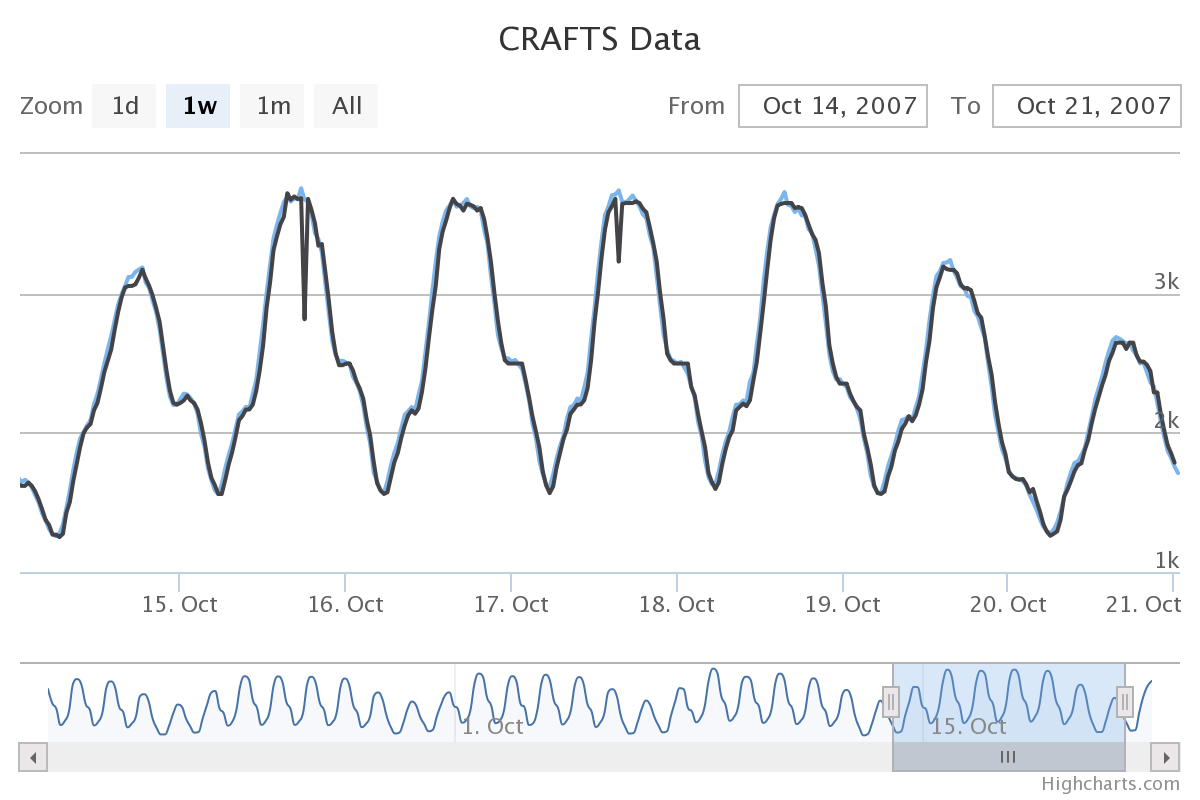
\includegraphics[width=\textwidth]{results/graphs/markov_baseline.png}
\caption{Markov prediction results for the baseline workload}
\label{fig:markov_b}
\end{figure}

\begin{table}[H]
\centering
\begin{tabular}{| l | l | l | l | l |}
\hline
Type & \multicolumn{2}{c |}{Regular} & \multicolumn{2}{c |}{Anomalous} \\ \hline
 & RMSD & Percent & RMSD & Percent \\ \hline
Under & 80 & 61.4\% & 7 & 18.2\% \\ \hline
Over & 61 & 38.6\% & 13 & 81.8\% \\ \hline
Total & 73 & & 13 & \\ \hline
\end{tabular}
\caption{Markov predictor results for the training outage workload}
\end{table}

\begin{figure}[H]
\centering
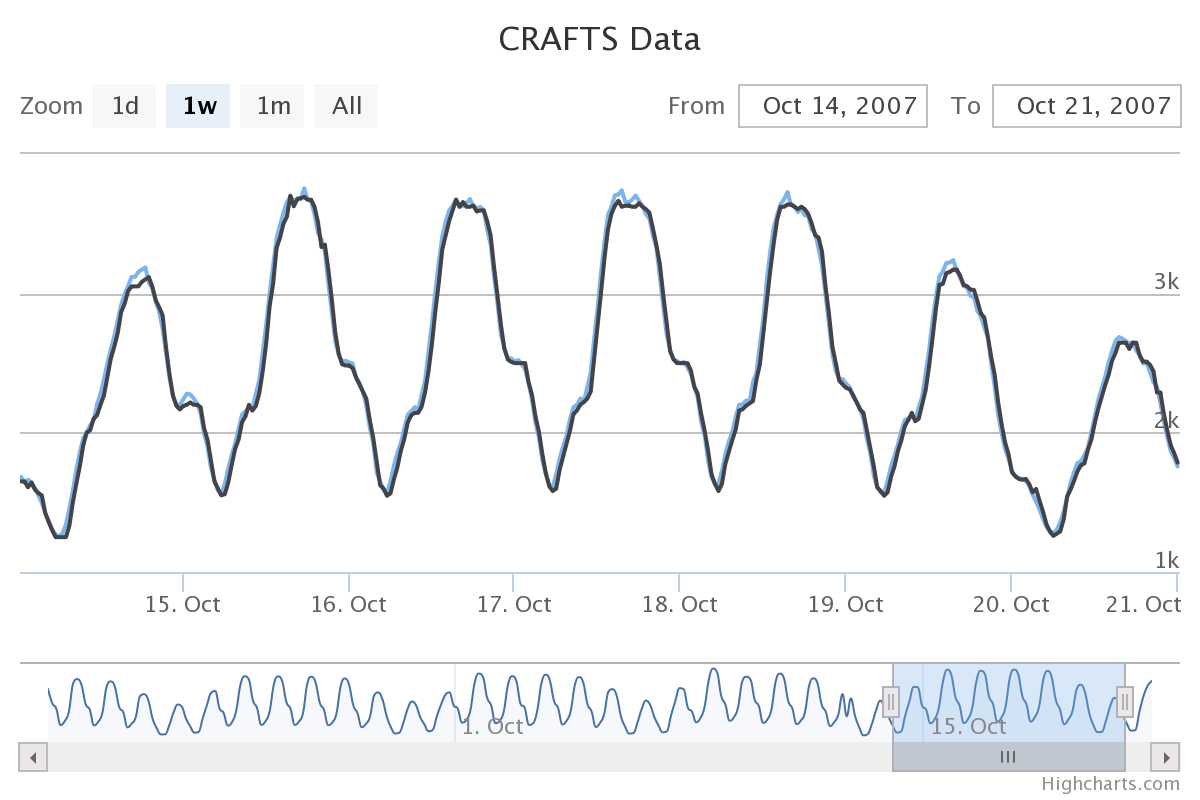
\includegraphics[width=\textwidth]{results/graphs/markov_training_outage.png}
\caption{Markov prediction results for the training outage workload}
\label{fig:markov_to}
\end{figure}

\begin{table}[H]
\centering
\begin{tabular}{| l | l | l | l | l |}
\hline
Type & \multicolumn{2}{c |}{Regular} & \multicolumn{2}{c |}{Anomalous} \\ \hline
 & RMSD & Percent & RMSD & Percent \\ \hline
Under & 211 & 59.4\% & 0 & 0.0\% \\ \hline
Over & 123 & 40.6\% & 1325 & 100.0\% \\ \hline
Total & 181 & & 1325 & \\ \hline
\end{tabular}
\caption{Markov predictor results for the horizon outage workload}
\end{table}

\begin{figure}[H]
\centering
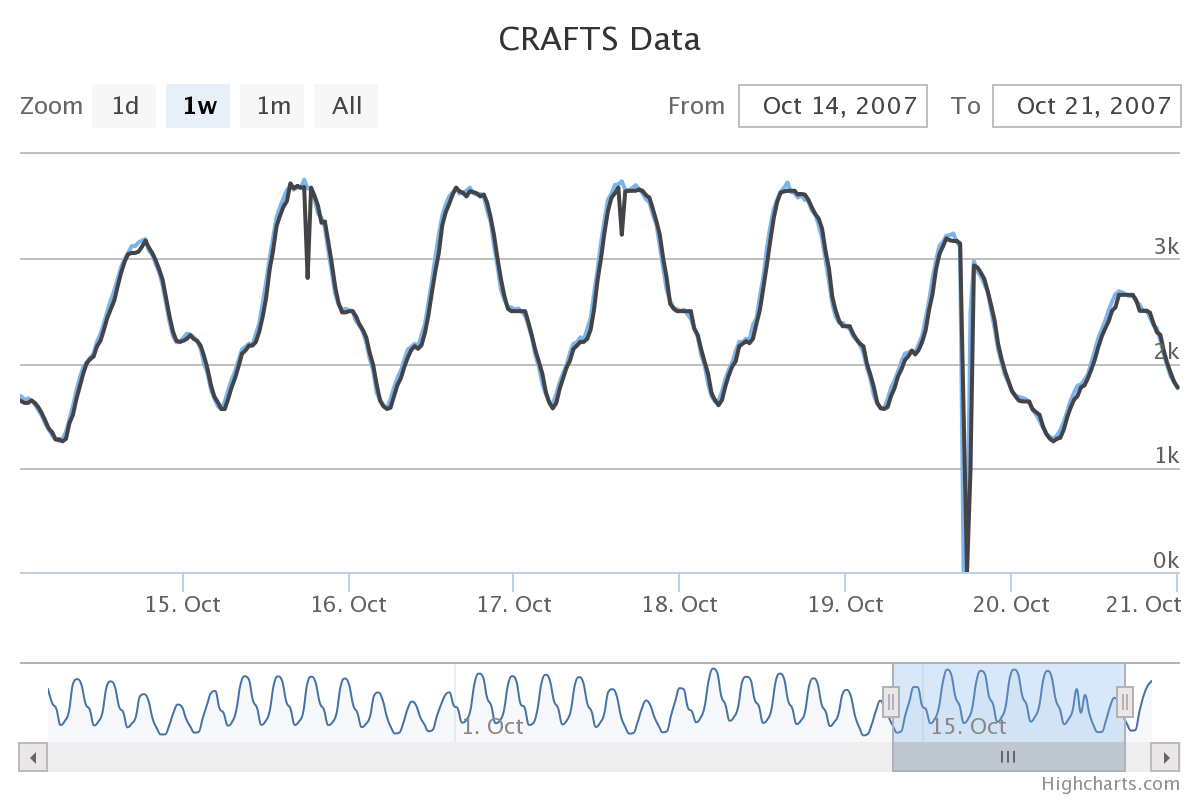
\includegraphics[width=\textwidth]{results/graphs/markov_horizon_outage.png}
\caption{Markov prediction results for the horizon outage workload}
\label{fig:markov_ho}
\end{figure}

\begin{table}[H]
\centering
\begin{tabular}{| l | l | l | l | l |}
\hline
Type & \multicolumn{2}{c |}{Regular} & \multicolumn{2}{c |}{Anomalous} \\ \hline
 & RMSD & Percent & RMSD & Percent \\ \hline
Under & 147 & 64.5\% & 0 & 0.0\% \\ \hline
Over & 62 & 35.5\% & 28 & 100.0\% \\ \hline
Total & 124 & & 28 & \\ \hline
\end{tabular}
\caption{Markov predictor results for the training spike workload}
\end{table}

\begin{figure}[H]
\centering
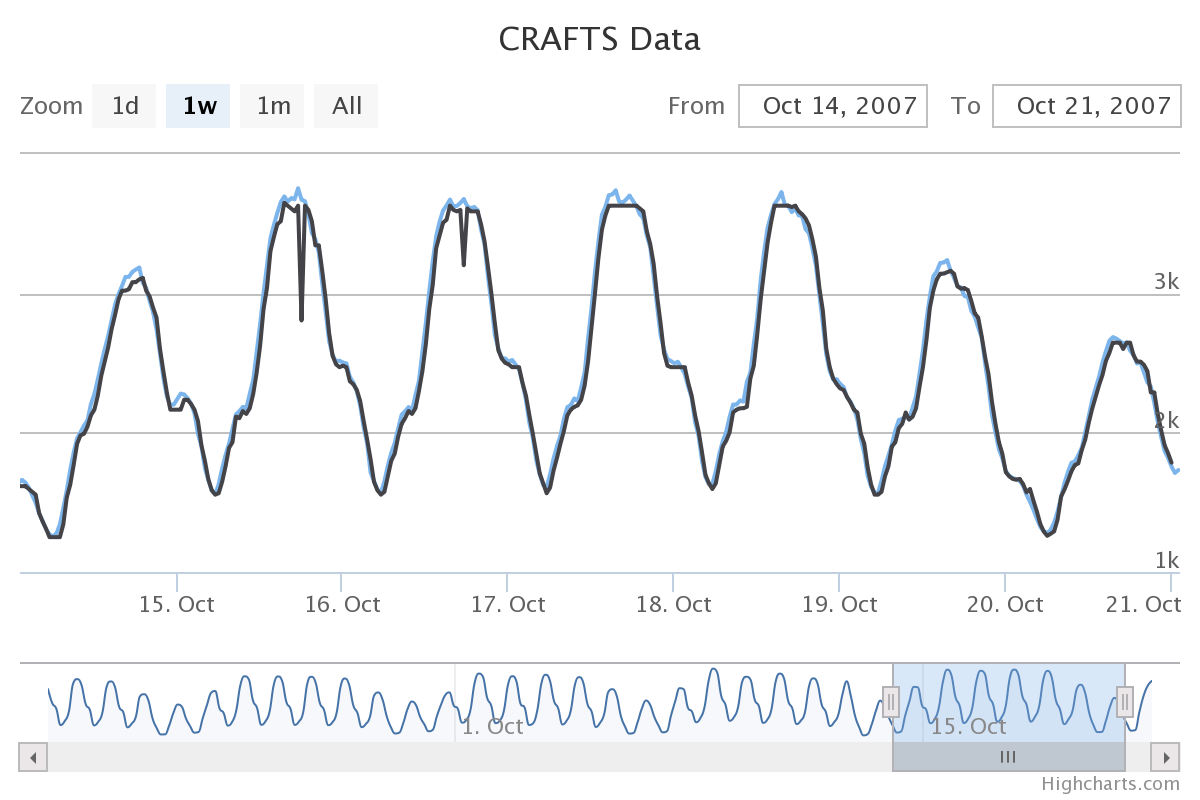
\includegraphics[width=\textwidth]{results/graphs/markov_training_spike.png}
\caption{Markov prediction results for the training spike workload}
\label{fig:markov_ts}
\end{figure}

\begin{table}[H]
\centering
\begin{tabular}{| l | l | l | l | l |}
\hline
Type & \multicolumn{2}{c |}{Regular} & \multicolumn{2}{c |}{Anomalous} \\ \hline
 & RMSD & Percent & RMSD & Percent \\ \hline
Under & 231 & 59.5\% & 2996 & 100.0\% \\ \hline
Over & 160 & 40.5\% & 0 & 0.0\% \\ \hline
Total & 205 & & 2996 & \\ \hline
\end{tabular}
\caption{Markov predictor results for the horizon spike workload}
\end{table}

\begin{figure}[H]
\centering
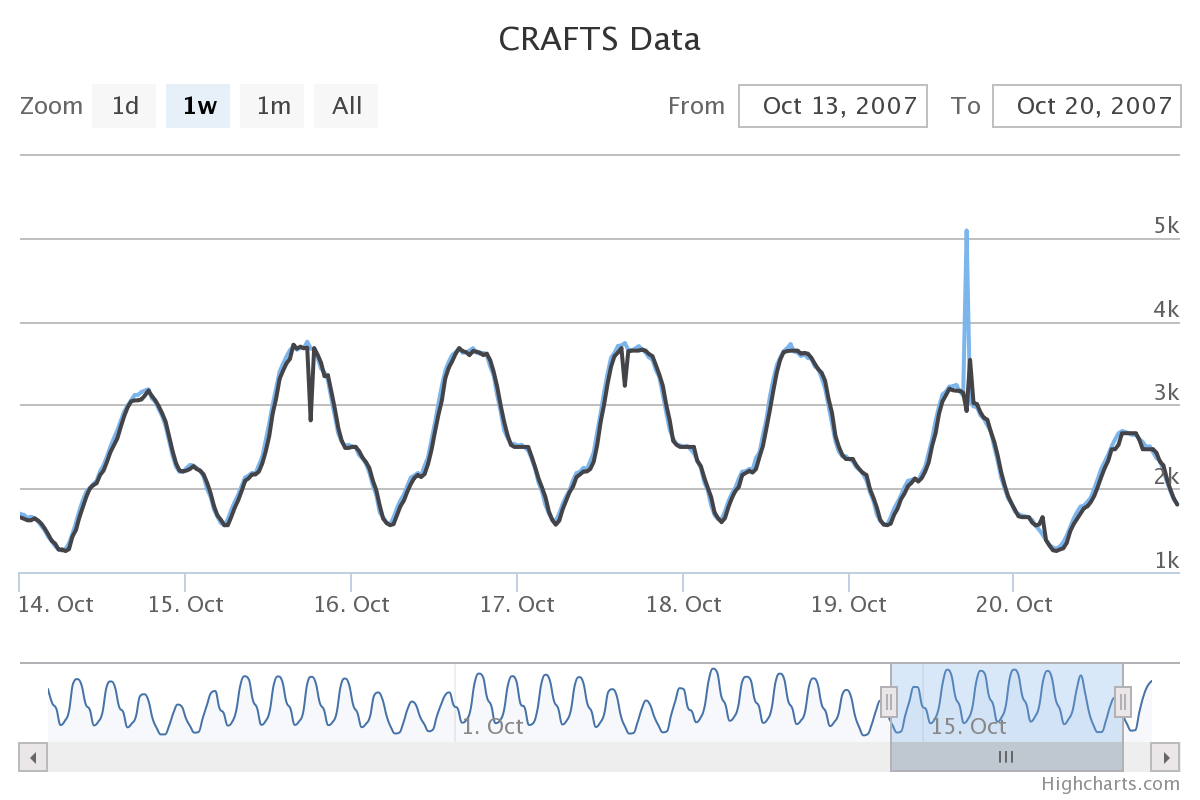
\includegraphics[width=\textwidth]{results/graphs/markov_horizon_spike.png}
\caption{Markov prediction results for the horizon spike workload}
\label{fig:markov_hs}
\end{figure}